\setcounter{chaptercntr}{5}

\sectionbreak \section*{
	\gostTitleFont
	\redline
	\thechaptercntr .
	РАЗВЁРТЫВАНИЕ МОДЕЛИ НЕЙРОННОЙ СЕТИ
}

\titlespace

\subsection*{ 
	\gostTitleFont
	\redline
	\thechaptercntr .\thesubchaptercntr \spc
	Основные виды развертывания
} \addtocounter{subchaptercntr}{1}

\subtitlespace

{\gostFont

	\par \redline Развертывание и работа являются одними из основных этапов жизни проекта. От успех на данном этапе зависит бесперебойное функционирование системы.

	\par \redline Есть несколько паттернов развертывания модели: статически, как часть устанавливаемого пакета, динамически на устройстве пользователя, динамически на сервере или потоком.

	\par \redline У статического развертывания много преимуществ, например быстрое выполнение, ненарушенная конфиденциальность пользователя и возможность обращаться к модели без подключения к сети. Есть и недостаток: труднее обновить модель без обновления всего приложения в целом.

	\par \redline Главное преимущество динамического развертывания на устройствах пользователей {--} быстрое обращение к модели. Кроме того, уменьшается нагрузка на серверы организации. Недостатки – трудность доставки обновлений всем пользователям и доступность модели для стороннего анализа.

	\par \redline Как и статическое развертывание, развертывание на устройстве пользователя затрудняет мониторинг качества модели.

	\par \redline Динамическое развертывание на сервере может принимать одну из следующих форм: развертывание на виртуальной машине, развертывание в контейнере и бессерверное развертывание.

	\par \redline Самый популярный способ {--} развернуть модель на сервере и сделать ее доступной с помощью REST API, раскрываемого веб-сервисом или службой gRPC. В этом случае клиент отправляет запрос серверу, а затем ждет ответа, прежде чем отправить следующий запрос.

	\par \redline Потоковое развертывание модели устроено иначе. Все модели регистрируются в движке потоковой обработки или упаковываются в виде приложения, основанного на библиотеке потоковой обработки. Клиент отправляет один запрос и получает обновления по мере их возникновения.

	\par \redline Типичные стратегии развертывания: разовое, немое, канареечное и многорукий бандит.

	\par \redline При разовом развертывании новая модель сериализуется в виде файла, затем старый файл заменяется новым.

	\par \redline  Немое развертывание подразумевает развертывание старой и новой версий и их параллельную работу. Новая версия не предъявляется пользователю, пока не произойдет переключение. Предсказания новой версии только записываются в журнал и анализируются. Поэтому остается достаточно времени, чтобы удостовериться в правильной работе новой модели, не беспокоя пользователей. Недостаток в том, что приходится выполнять больше моделей, расходуя дополнительные ресурсы.

	\par \redline  Канареечное развертывание заключается в том, что новая версия отправляется небольшой доле пользователей, а большинство продолжает работать со старой версией. Это позволяет проверить качество модели и оценить ее удобство для пользователей. В случае ошибки пострадает не так много пользователей.

	\par \redline  Многорукие бандиты позволяют развернуть новую модель, оставив старую. Алгоритм заменяет старую модель новой, только когда уверен, что новая работает лучше.

	\par \redline Развертывание новой версии модели должно быть автоматизированным и транзакционным. Получив номер версии подлежащей развертыванию модели, скрипт извлекает модель и экстрактор признаков из соответствующих репозиториев и копирует их в производственную среду. Модель должна быть применена к сквозным и доверительным тестовым данным путем имитации вызова извне. Если на сквозных данных возникает ошибка предсказания или на доверительных данных значение метрики качества выходит за пределы допустимого диапазона, то все развертывание следует откатить.

	\par \redline Версии обучающих данных, экстрактора признаков и модели должны быть синхронизированы.

	\par \redline Эффективность алгоритмов {--} важный аспект развертывания модели.	Python пакеты для научных расчетов: NumPy, SciPy, scikit-learn и др. {--} написаны опытными учеными и инженерами, которые уделяли большое внимание эффективности. Ваш собственный код может оказаться не таким эффективным и надежным. Писать свой код следует, только если это абсолютно необходимо.

	\par \redline При реализации собственного алгоритма избегайте циклов. Используйте подходящие структуры данных. Если порядок элементов коллекции не играет роли, используйте множество вместо списка. Использование словарей (или хеш-таблиц) позволяет определить коллекцию пар ключ–значение, в которой поиск ключа производится очень быстро.

	\par \redline Кеширование ускоряет приложение, если оно содержит ресурсоемкие функции, которые часто вызываются с одними и теми же параметрами. В машинном обучении такими ресурсоемкими функциями являются модели, особенно исполняемые на GPU.

	\par \redline В данном случае будет осуществляться статическое развертывание. Подобное разветрывание обеспечит безопасность и высокое быстродействие, что является основными характеристиками, которые необходимы от разрабатываемой нейронной.[6]

	\par
}

\subtitlespace

\subsection*{
	\gostTitleFont
	\redline
	\thechaptercntr .\thesubchaptercntr \spc
	Технология PCLNext и контроллер AXC F 2152
} \addtocounter{subchaptercntr}{1}

\subtitlespace

{\gostFont

	\par \redline Нейронная сеть будет разворачиваться на контроллерах PCLnext.

	\par \redline PLCnext Control {--} это аппаратное обеспечение технологии PLCnext, предлагающее открытую среду Linux с доступом к большему количеству данных через системы интернета вещей и большей гибкостью. В дополнение к таким стандартам, как IEC 61131, параллельное программирование и комбинация языков программирования, таких как C / C++, C\# или MATLAB® Simulink®, также возможны в режиме реального времени с помощью PLCnext Control. Существуют три различные категории управления PLCnext: гибкие модульные контроллеры, высокопроизводительные удаленные полевые контроллеры и контроллеры на базе iPC.[13]

	\par \redline Данные преимущества платформы PLCnext в совокупности с преимуществами выбранного метода развертывания позволяют говорить о возможности дальнейшего эффективного применения разработанной нейронной сети.

	\par \redline В качестве управляющего устройства в данном проекте используется PLCNext-Technology Starterkit  рисунке \thechaptercntr.\theimagecntr. Это комплект, включающий все необходимое для работы с технологией PLCNext для промышленной автоматизации. В комплект входит устройство управления {--} контроллер AXC F 2152, модули ввода/вывода AXL Smart Elements DI16/DO16/AI4, ползунковый потенциометр, Ethernet-кабель для подключения, книга стартового набора и ссылка на файл моделирования. Комплект разработан для обеспечения простого, удобного и экономически эффективного способа начать проекты с использованием технологии PLCNext. С помощью этого набора пользователи могут опробовать принцип работы, управление и высокую производительность технологии PLCNext на малогабаритной станции. PLCNext StarterKit сопровождается подробной документацией и руководством пользователя, которые помогают быстро разобраться с платформой и начать разработку. Также может быть предоставлен доступ к онлайн-курсам и материалам для дополнительного обучения и погружения в возможности PLCNext.[14]

	\begin{figure}[H]
		\centering
		\def\svgwidth{\textwidth}
		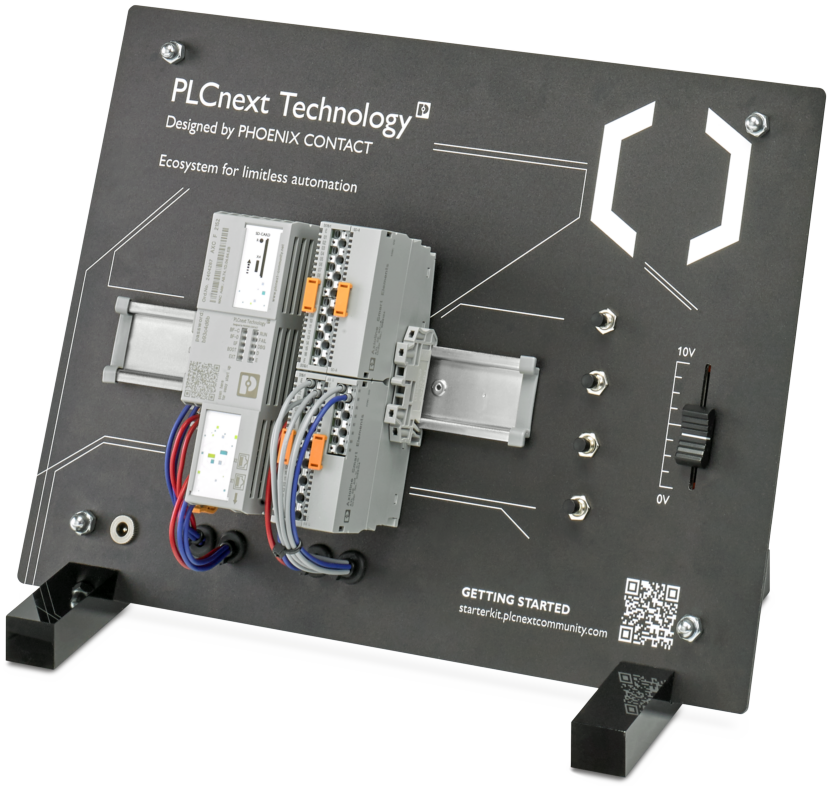
\includegraphics[scale=0.7]{images/pclnext_x.png}
		\caption*{\gostFont Рисунок \thechaptercntr .\theimagecntr \spc {--} PLCNext-Technology Starterkit}
		\label{fig:ACXF2152}
	\end{figure}  \addtocounter{imagecntr}{1}

	\par \redline Остановимся подробнее на «сердце» платформы {--} контроллере AXC F 2152. Контроллер обладает мощными вычислительными возможностями, различными интерфейсами ввода-вывода и поддержкой различных языков программирования.[14]

	\par \redline Подробные технические характеристики контроллера AXC F 2152:

	\begin{itemize}[leftmargin=2.15cm, labelwidth=0.65cm, labelsep=0.0cm] 

		\item[\theitemcntr. ] Процессор:
			\begin{itemize}[leftmargin=1.5cm, labelwidth=0.65cm, labelsep=0.0cm] 
				\item[•] Процессор: 2-ядерный ARM Cortex-A9.
				\item[•] Частота процессора: 800 МГц.
				\item[•] Встроенная память: 1 ГБ RAM, 4 ГБ eMMC.
			\end{itemize} \addtocounter{itemcntr}{1}

		\item[\theitemcntr. ] Коммуникационные интерфейсы:
			\begin{itemize}[leftmargin=1.5cm, labelwidth=0.65cm, labelsep=0.0cm] 
				\item[•] Ethernet: 2 x 10/100/1000 Мбит/с.
				\item[•] USB: 2 x USB 2.0 Host.
				\item[•] RS232: 1 x порт с поддержкой RTS/CTS.
			\end{itemize} \addtocounter{itemcntr}{1}

		\item[\theitemcntr. ] Входы/выходы:
			\begin{itemize}[leftmargin=1.5cm, labelwidth=0.65cm, labelsep=0.0cm] 
				\item[•] Цифровые входы: 16 x 24 В постоянного тока, с поддержкой функции счетчика.
				\item[•] Цифровые выходы: 16 x 24 В постоянного тока, максимальный ток 500 мА на выход.
				\item[•] Аналоговые входы: 2 x 0-10 В, 12-битное разрешение.
				\item[•] Аналоговые выходы: 2 x 0-10 В, 12-битное разрешение.
			\end{itemize} \addtocounter{itemcntr}{1}

		\item[\theitemcntr. ] Расширение:
			\begin{itemize}[leftmargin=1.5cm, labelwidth=0.65cm, labelsep=0.0cm] 
				\item[•] Слоты для расширения: 2 x слоты для модулей расширения PLCNext.
				\item[•] Поддержка модулей расширения: Модули ввода-вывода, модули интерфейсов связи и дополнительные функциональные модули.
			\end{itemize} \addtocounter{itemcntr}{1}

		\item[\theitemcntr. ] Питание:
			\begin{itemize}[leftmargin=1.5cm, labelwidth=0.65cm, labelsep=0.0cm] 
				\item[•] Напряжение питания: 24 В постоянного тока.
				\item[•] Потребляемая мощность: максимально 18 Вт.
		    \end{itemize} \addtocounter{itemcntr}{1}

		\item[\theitemcntr. ] Операционная система:
			\begin{itemize}[leftmargin=1.5cm, labelwidth=0.65cm, labelsep=0.0cm] 
				\item[•] PLCNext Runtime: Основан на операционной системе Linux.
			\end{itemize} \addtocounter{itemcntr}{1}

		\item[\theitemcntr. ] Программное обеспечение:
			\begin{itemize}[leftmargin=1.5cm, labelwidth=0.65cm, labelsep=0.0cm] 
				\item[•] Поддерживаемые языки программирования: IEC 61131-3 (ST, LD, FBD, SFC), C++, C\#, Python.
				\item[•] Встроенное ПО: PLCNext Engineer, PLCNext Runtime.
			\end{itemize} \addtocounter{itemcntr}{1}

		\item[\theitemcntr. ] Рабочие условия:
			\begin{itemize}[leftmargin=1.5cm, labelwidth=0.65cm, labelsep=0.0cm] 
				\item[•] Рабочая температура: от 0°C до 55°C.
				\item[•] Влажность: от 5\% до 95\%, без конденсации.
			\end{itemize} \addtocounter{itemcntr}{1}

	\end{itemize} \setcounter{itemcntr}{1}

	\par \redline Основные компоненты контроллера AXC F 2152 (модули, интерфейсы) отражены на рис. \thechaptercntr.\theimagecntr. 

	\begin{figure}[H]
		\centering
		\def\svgwidth{\textwidth}
		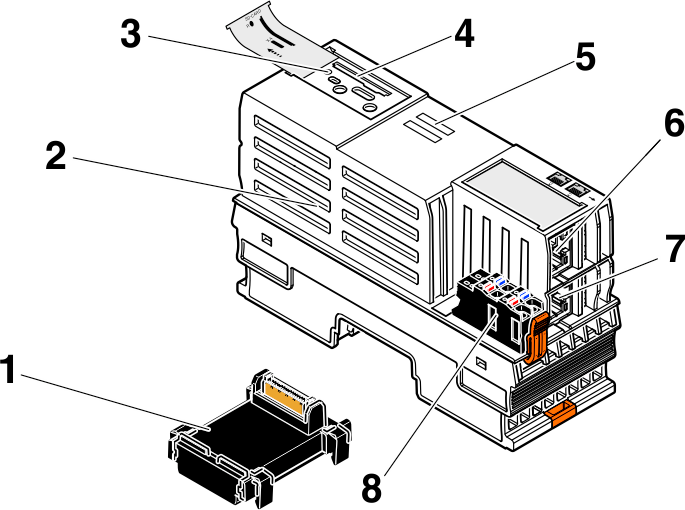
\includegraphics[scale=1.8]{images/pclnext_complect.png}
		\caption*{\gostFont Рисунок \thechaptercntr .\theimagecntr \spc {--} Компоненты контроллера AXC F 2152}
		\label{fig:PLCComplect}
	\end{figure} \addtocounter{imagecntr}{1}

	\par \redline Где на контроллере:

	\begin{itemize}[leftmargin=2.15cm, labelwidth=0.65cm, labelsep=0.0cm] 

		\item[\theitemcntr. ] Базовый модуль шины.
		\addtocounter{itemcntr}{1}

		\item[\theitemcntr. ] Модуль электроники.
		\addtocounter{itemcntr}{1}

		\item[\theitemcntr. ] Кнопка сброса.
		\addtocounter{itemcntr}{1}

		\item[\theitemcntr. ] Держатель SD-карты.
		\addtocounter{itemcntr}{1}

		\item[\theitemcntr. ] Индикаторы диагностики и состояния.
		\addtocounter{itemcntr}{1}

		\item[\theitemcntr. ] Интерфейс Ethernet (1).
		\addtocounter{itemcntr}{1}

		\item[\theitemcntr. ] Интерфейс Ethernet (2).
		\addtocounter{itemcntr}{1}

		\item[\theitemcntr. ] Разъем для подключения напряжения питания.
		\addtocounter{itemcntr}{1}

	\end{itemize} \setcounter{itemcntr}{1}

	\par \redline Для подключения различной периферии к контроллеру AXC F 2152 необходимо:

	\begin{itemize}[leftmargin=2.15cm, labelwidth=0.65cm, labelsep=0.0cm] 

		\item[\theitemcntr. ] Использовать модуль базовой шины для соединения контроллера с локальной шиной Axioline F, к которой можно подключить до 63 устройств ввода-вывода.
		\addtocounter{itemcntr}{1}

		\item[\theitemcntr. ] Использовать интерфейс(ы) Ethernet для подключения контроллера.
		\addtocounter{itemcntr}{1}

		\item[\theitemcntr. ] Настроить параметры сети и контроллера.
		\addtocounter{itemcntr}{1}

		\item[\theitemcntr. ] Создать новый проект, добавить контроллер и периферийные устройства в конфигурацию оборудования.
		\addtocounter{itemcntr}{1}

		\item[\theitemcntr. ] Загрузить проект в контроллер и запустить его.
		\addtocounter{itemcntr}{1}

	\end{itemize} \setcounter{itemcntr}{1}

	\par \redline К контроллеру AXC F 2152 можно подключить различные устройства ввода-выво- да системы Axioline F, такие как:

	\begin{itemize}[leftmargin=2.15cm, labelwidth=0.65cm, labelsep=0.0cm] 

		\item[\theitemcntr. ] Цифровые модули ввода-вывода (например, DI8/1 DO8/1 2701916) для работы с дискретными сигналами. 
		\addtocounter{itemcntr}{1}

		\item[\theitemcntr. ] Аналоговые модули ввода-вывода (например, AI2 AO2 2702072) для работы с аналоговыми сигналами. 
		\addtocounter{itemcntr}{1}

		\item[\theitemcntr. ] Модули специального назначения (например, AXF BK PN 2701815) для подключения к другим шинам.
		\addtocounter{itemcntr}{1}

	\end{itemize} \setcounter{itemcntr}{1}

	\par \redline Контроллер AXC F 2152 PLCNext Control обладает высокой производительностью, разнообразными интерфейсами связи, расширяемостью и поддержкой различных языков программирования. Он идеально подходит для автоматизации производственных процессов, обеспечивая гибкость, надежность и удобство разработки.

	\par
}

\subtitlespace

\subsection*{
	\gostTitleFont
	\redline
	\thechaptercntr .\thesubchaptercntr \spc
	Выбор средств сборки под контроллер на платформе PCLNext
} \addtocounter{subchaptercntr}{1}

\subtitlespace

{\gostFont
	
	\par \redline Нейронная сеть была разработана на платформе Window в Visual Studio 2022. Для успешного развертывания на контроллерах PCLnext необходимо собрать данные проекты для данной платформы.
	
	\par \redline Это мощная и популярная интегрированная среда разработки (IDE) от компании Microsoft. Преимущества, по совокупности которых было решено остановиться на этом инструменте, как наиболее подходящем для решения поставленных задач:
	
	\begin{itemize}[leftmargin=2.15cm, labelwidth=0.65cm, labelsep=0.0cm] 

		\item[\theitemcntr. ] Богатый функционал. Visual Studio Community обладает широким набором инструментов и возможностей, которые помогут разрабатывать и отлаживать программное обеспечение. Она поддерживает различные языки программирования, включая C++, C\#, Visual Basic, Python и многие другие, которые можно использовать с PLCNext SDK. Также в состав Visual Studio входят мощные инструменты для отладки, профилирования, управления версиями и автоматизации разработки.
		\addtocounter{itemcntr}{1}

		\item[\theitemcntr. ] Интеграция с другими инструментами. Visual Studio Community интегрируется с различными сервисами и инструментами разработки, что облегчает работу с ними. Visual Studio имеет расширение PLCNext Technology Development Tools, которое добавляет шаблоны проектов и элементов, а также модуль отладки для PLCNext Technology. VS также поддерживает CMake, который является системой сборки для настоящего проекта.
		\addtocounter{itemcntr}{1}
		
		\item[\theitemcntr. ] Доступность. Visual Studio Community предоставляется бесплатно для некоммерческого использования, включая академические и личные проекты. Это позволяет сэкономить средства на лицензировании среды разработки
		\addtocounter{itemcntr}{1}
		
		\setcounter{itemcntr}{1}
	\end{itemize} 	

	\par \redline Для программирования контроллера будет использован PLC Toolchain. Это набор инструментов для программирования контроллеров логического управления на высокоуровневых языках, таких как C++ и C\#. Это помогает использовать возможности этих языков для создания сложных и эффективных алгоритмов управления, а также для интеграции с другими системами и технологиями.

	\par \redline PLC Toolchain основан на среде разработки Beremiz, которая соответствует стандарту IEC 61131-3. Этот стандарт определяет пять языков программирования для PLC: Instruction list, Symbolic flowchart, Ladder diagram, Function block diagram и Structured text. PLC Toolchain позволяет использовать эти языки в сочетании с C++ и C\#, а также переносить код между разными платформами и аппаратным обеспечением.

	\par \redline PLC Toolchain включает в себя инструменты для создания HMI (Human-Machine Interface), а также для подключения программ PLC к существующим базам данных и полевым шинам. 

	\par \redline Также для работы с платформой PLCNext и контроллером AXC F 2152 необходимо будет использовать PLCNext SDK – набор инструментов для разработки приложений для контроллеров PLCNext Technology на разных языках программирования. PLCNext SDK включает в себя компиляторы, отладчики, библиотеки и другие ресурсы, необходимые для создания нативных приложений для целевого устройства. PLCNext SDK устанавливается и управляется с помощью командной строки (CLI), называемой PLCNext CLI или plcncli.

	\par
}

\subtitlespace

\subsection*{ 
	\gostTitleFont
	\redline
	\thechaptercntr .\thesubchaptercntr \spc
	Выбор средств установки программ на платформу PCLNext
} \addtocounter{subchaptercntr}{1}

\subtitlespace

{\gostFont

	\par \redline После сборки нейронной сети необходимо перенести полученный исполняемый файл на имеющийся контроллер.

	\par \redline Для подобной задачи можно использовать несколько вариантов:

	\begin{itemize}[leftmargin=2.15cm, labelwidth=0.65cm, labelsep=0.0cm] 

		\item[\theitemcntr. ]	Программу WinSCP в связке с программой Putty 64-bit. 
		\addtocounter{itemcntr}{1}

		\item[\theitemcntr. ] Специализированные программные средства PLCNext Engineer. 
		\addtocounter{itemcntr}{1}

	\end{itemize} \setcounter{itemcntr}{1}

	\par \redline Данные средства обладают своими плюсами и недостатками. Опишем их. 

	\par \redline Основным плюсом PLCNext Engineer является её приспособленность конкретно к технологии PLCNext. PLCnext Engineer - это программный комплекс для разработки автоматизированных решений на основе контроллеров. Он включает в себя все инженерные дисциплины, необходимые для полной разработки и ввода в эксплуатацию прикладного проекта по автоматизации. Эти инженерные задачи включают в себя:

	\begin{itemize}[leftmargin=2.15cm, labelwidth=0.65cm, labelsep=0.0cm] 

		\item[\theitemcntr. ] Создание сетей.
		\addtocounter{itemcntr}{1}

		\item[\theitemcntr. ] Разработка прикладного кода.
		\addtocounter{itemcntr}{1}
		
		\item[\theitemcntr. ] HMI (Человеко-машинный интерфейс).
		\addtocounter{itemcntr}{1}

		\item[\theitemcntr. ] Сервер OPC UA.
		\addtocounter{itemcntr}{1}

	\end{itemize} \setcounter{itemcntr}{1}

	\par \redline Данные функции позволяют утверждать о высокой приспособленности PLCNext Engineer для внедрения разработанной программы в контроллер.

	\par \redline Однако, PLCNext Engineer не является единственной альтернативой. Для полноценного выбора следует рассмотреть возможность применения иных программ, таких как PuTTY в связке с WinSCP.

	\par \redline PuTTY {--} это SSH- и telnet-клиент, первоначально разработанный Саймоном Татхэмом для платформы Windows. PuTTY {--} это программное обеспечение с открытым исходным кодом, доступное с исходным кодом и разрабатываемое и поддерживаемое группой добровольцев.

	\par \redline WinSCP {--} это бесплатный SFTP-клиент с открытым исходным кодом, FTP-клиент, клиент WebDAV, клиент S3 и клиент SCP и файловый менеджер для Windows. Его основная функция - передача файлов между локальным и удаленным компьютерами. Помимо этого, WinSCP предлагает сценарии и базовые функции файлового менеджера.

	\par \redline WinSCP предоставляет:

	\begin{itemize}[leftmargin=2.15cm, labelwidth=0.65cm, labelsep=0.0cm] 

		\item[•] 	Графический пользовательский интерфейс.  
		\addtocounter{itemcntr}{1}

		\item[•] Среду на многих языках.
		\addtocounter{itemcntr}{1}

		\item[•] Интеграция с Windows (перетаскивание, URL, значки быстрого доступа, список переходов). 
		\addtocounter{itemcntr}{1}

		\item[•] Все распространенные операции с файлами, как удаленные, так и локальные.  
		\addtocounter{itemcntr}{1}

		\item[•] Поддержка протоколов SFTP и SCP через SSH и FTP, WebDAV,S3. 
		\addtocounter{itemcntr}{1}

		\item[•]  Командный файл скриптовый интерфейс и командная строка и .NET assembly для сложных задач программирования.
		\addtocounter{itemcntr}{1}

		\item[•] Синхронизация каталогов несколькими полуавтоматическими способами 
		\addtocounter{itemcntr}{1}

		\item[•] Встроенный текстовый редактор
		\addtocounter{itemcntr}{1}

		\item[•] Предоставляет общий доступ к настройкам сайта с помощью PuTTY 
		\addtocounter{itemcntr}{1}

		\item[•] Поддержка аутентификации с использованием пароля, клавиатуры, открытого ключа и Kerberos (GSS). 
		\addtocounter{itemcntr}{1}

		\item[•] Интегрируется с Pageant (PuTTY authentication agent) для полной поддержки аутентификации с открытым ключом по SSH.
		\addtocounter{itemcntr}{1}

		\item[•] Проводник и менеджер интерфейсов. 
		\addtocounter{itemcntr}{1}

		\item[•] Опционально защищает сохраненную информацию сайта с помощью мастер-пароля.
		\addtocounter{itemcntr}{1}

		\item[•] Опционально поддерживает переносимую работу с использованием файла конфигурации вместо записей реестра, подходящего для работы со съемных носителей.
		\addtocounter{itemcntr}{1}

	\end{itemize} \setcounter{itemcntr}{1}	

	\par \redline В рамках дипломного проекта было решено остановиться на PuTTY в связке с WinSCP. 

    \par \redline Данное решение было принято в связи с простотой программ, большим функционалом и возможностью связки данных программ покрыть собой все возможные потребности по переносу собранного исполняемого файла нейронной сети на контроллер.

	\par
}

\subtitlespace

\subsection*{
	\gostTitleFont
	\redline
	\thechaptercntr .\thesubchaptercntr \spc
	Портирование программы на контроллер
} \addtocounter{subchaptercntr}{1}

\subtitlespace

{\gostFont

	\par \redline Для успешной сборки существующей программы на контроллер будут использоваться следующие компоненты[15]:

	\begin{itemize}[leftmargin=2.15cm, labelwidth=0.65cm, labelsep=0.0cm] 

		\item[\theitemcntr. ] CMake (система сборки).
		\addtocounter{itemcntr}{1}

		\item[\theitemcntr. ] PLCNCLI (командная строка для контроллеров PLCNext).
        \addtocounter{itemcntr}{1}

		\item[\theitemcntr. ] SDK для выбранного контроллера.
        \addtocounter{itemcntr}{1}		

		\setcounter{itemcntr}{1}
	\end{itemize}

	\par \redline Для успешной сборки программы под выбранный контроллер необходимо установить CMake на компьютер. Данная среда обеспечит возможность кроссплатформенной сборки на разные платформы.

	\par \redline После успешной установки CMake, необходимо установить на компьютер командную строку PLCNCLI для возможности установки выбранных SDK и сборки программ под выбранный контроллер. Она обеспечит установки необходимых инструментов для сборки программы.

	\par \redline После успешной установки PLCNCLI, необходимо скачать с официального сайта и установить на компьютер SDK через командную строку PLCNCLI командой: plcncli.exe install sdk –d [installation path] –p [path to archive file].  После установки SDK необходимо переходить в Visual Studio и настраивать проект CMake по контроллер.
	\par \redline На рисунке \thechaptercntr .\theimagecntr \spc показан первый этап работы программы {--} загрузка данных. В ходе этого этапа сеть не даёт результаты, а формирует входную цепочку данных для подачи её на сеть. А пока этой цепочки нет, то на сеть ничего не подаётся. 

	\begin{figure}[H]
		\centering
		\def\svgwidth{\textwidth}
		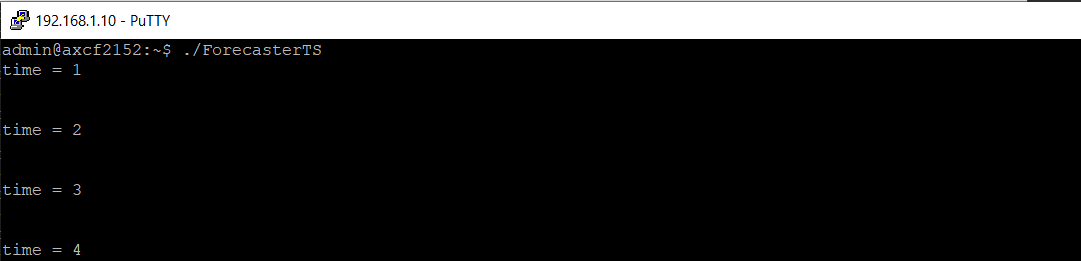
\includegraphics[width=\textwidth]{images/ResultsDumping.png}
		\caption*{\gostFont Рисунок \thechaptercntr .\theimagecntr \spc {--} Начало работы модуля ForecasterTS}
		\label{fig:ResultsDumping}
	  \end{figure} \addtocounter{imagecntr}{1}

	\par \redline После наступает второй этап работы сети {--} формирование прогнозов на основе входных данных. Данный этап изображён на рисунке \thechaptercntr .\theimagecntr. 

	\begin{figure}[H]
		\centering
		\def\svgwidth{\textwidth}
		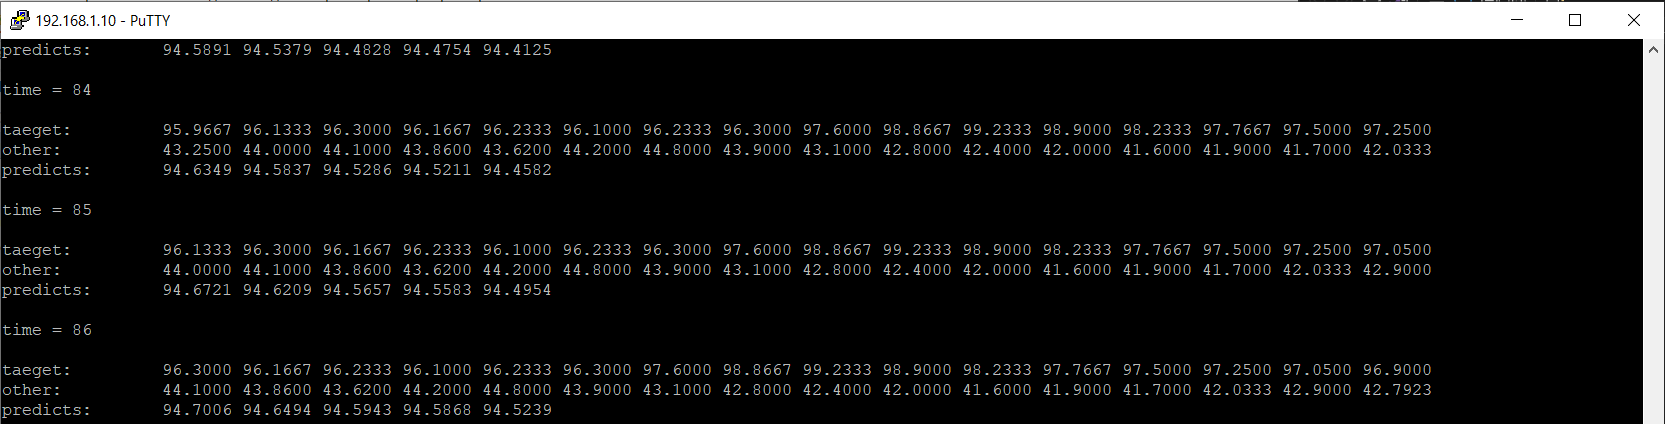
\includegraphics[width=\textwidth]{images/ResultsPredicts.png}
		\caption*{\gostFont Рисунок \thechaptercntr .\theimagecntr \spc {--} Формирование прогнозов на контроллере}
		\label{fig:ResultsPredicts}
	  \end{figure} \addtocounter{imagecntr}{1}

	\par
}

\setcounter{subchaptercntr}{1}
\setcounter{formulacntr}{1}
\setcounter{imagecntr}{1}
\setcounter{tablecntr}{1}
\setcounter{itemcntr}{1}
